\chapter{Volume Rendering}
\label{cap:vis_vol}

For volume rendering models, InVesalius employs a technique known as raycasting. Raycasting is a technique that simulates the trace of a beam of light toward the object through each screen pixel. The pixel color is based on the color and transparency of each voxel intercepted by the light beam.

InVesalius contains several pre-defined patterns (presets) to display specific tissue types or different types of exam (tomographic contrast, for example).

To access this feature, simply click the shortcut shown in Figure~\ref{fig:volume_raycasting_origina} in the lower right corner of the screen (next to the surfaces display window) and select one of the available presets.

To turn off volume rendering, click again on the path indicated by Figure~\ref{fig:volume_raycasting_origina} and select the \textbf{Disable} option.

\begin{figure}[!htb]
\centering
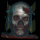
\includegraphics[scale=0.4]{volume_raycasting_origina}
\caption{Shortcut to volume visualization}
\label{fig:volume_raycasting_origina}
\end{figure}

\section{Viewing Standards}

There are several predefined viewing patterns. Some examples are illustrated in the following figures.

\begin{figure}[!htb]
\centering
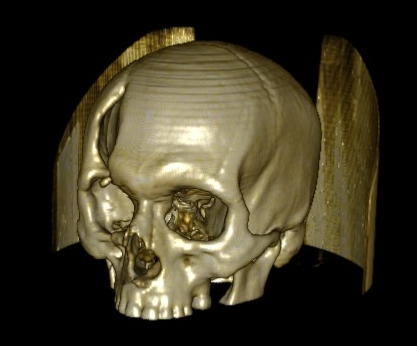
\includegraphics[scale=0.68]{brilhante_I}
\caption{Bright}
\label{fig:brilhante_I}
\end{figure}

\begin{figure}[!htb]
\centering 
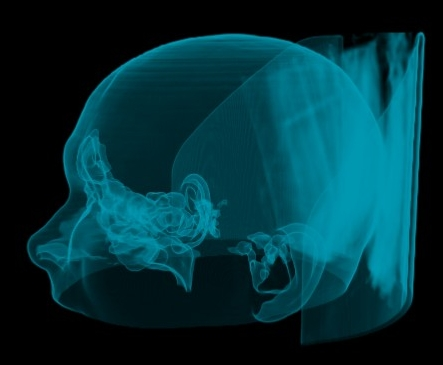
\includegraphics[scale=0.65]{vias_aereas_II}
\caption{Airway II}
\label{fig:vias_aereas_II} 
\end{figure}

\begin{figure}[!htb]
\centering
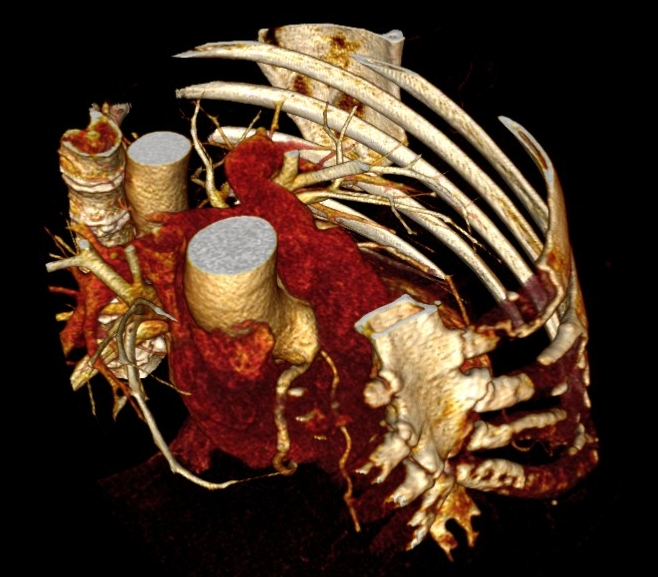
\includegraphics[scale=0.42]{contraste_medio}
\caption{Contrast Medium}
\label{fig:contraste_medio}
\end{figure}

\begin{figure}[!htb]
\centering
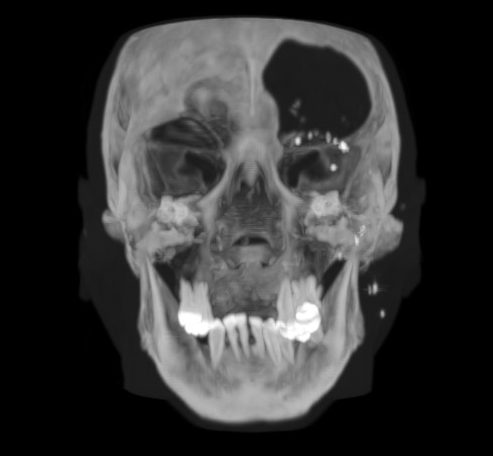
\includegraphics[scale=0.55]{MIP}
\caption{MIP}
\label{fig:MIP}
\end{figure}

\newpage

\section{Standard Customization}

Some patterns can be personalized (and customized). Figure~\ref{fig:customize_1} is exhibiting a pattern and some graphical controls adjustment. With these features, the color of a given structure and its opacity can be altered, determining if and how it will be displayed.

\begin{figure}[!htb]
\centering
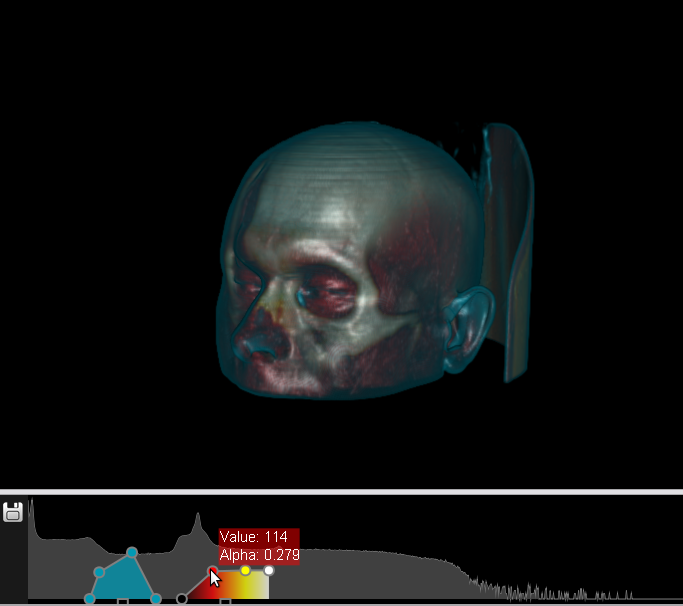
\includegraphics[scale=0.6]{customize_1}
\caption{Settings for the display pattern Soft Skin + II}
\label{fig:customize_1}
\end{figure}


\newpage

To hide a structure, use the control setting chart to decrease the opacity of the corresponding region. In the example in Figure~\ref{fig:customize_1} suppose we want to hide the muscular part (appearing in red). To do this, simply position the pointer over the muscular part in red and, using the left mouse button, drag the point down to reduce opacity and make the part transparent. Figure~\ref{fig:customize_2} illustrates the result.

Note: The Alpha value indicates the opacity of the color and the \textbf{value}, the color intensity of the pixel.

\begin{figure}[!htb]
\centering
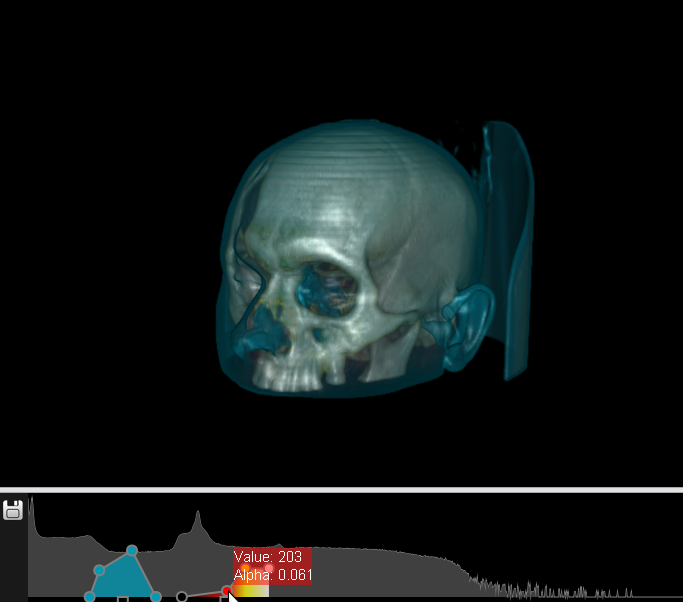
\includegraphics[scale=0.6]{customize_2}
\caption{Display Standard Soft Skin + II changed}
\label{fig:customize_2}
\end{figure}


\newpage

We can also remove or add points on the graph control setting. To remove, simply click with the right mouse button on the point. To add a new point, click the left button on the line graph. One can also save the resulting pattern by clicking the shortcut shown in Figure~\ref{fig:save_preset}.

\begin{figure}[!htb]
\centering

\includegraphics[scale=0.6]{save_preset}
\caption{Shortcut to save standard}
\label{fig:save_preset}
\end{figure}
 
To save the pattern, InVesalius displays a window like the one shown in Figure~\ref{fig:save_window_preset}. Enter a name for the custom pattern and \textbf{click OK}. The saved pattern will be available for the next time the software is opened.

\begin{figure}[!htb]
\centering
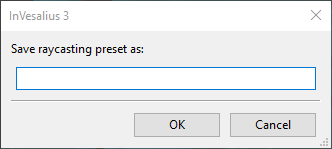
\includegraphics[scale=0.7]{save_window_preset_en.png}
\caption{Window to save name of pattern.}
\label{fig:save_window_preset}
\end{figure}

\section{Standard Customization with Brightness and Contrast}

You can customize a pattern without using the graphical control settings presented in the previous section. This is done through the \textbf{brightness and contrast} controls on the toolbar. Activate these by clicking the icon shown in Figure~\ref{fig:tool_contrast_original_vol}.

\begin{figure}[!htb]
\centering

\includegraphics[scale=0.6]{tool_contrast_original}
\caption{Shortcut to Brightness and Contrast}
\label{fig:tool_contrast_original_vol}
\end{figure}

Enable the control by dragging the mouse, with the left button pressed on the volume window. This will change the values of the window width and window level. The procedure is the same as with slices applied to 2D images, which can be seen in section~\ref{sec:ww_wl}. Dragging the mouse in a horizontal direction changes the window level value; drag left to decrease and right to increase. Dragging the mouse vertically changes the value of window width; drag down to decrease and up to increase.

Manipulating these values can be useful for different viewing results. For example, to add tissue to the display, \textbf{drag} the mouse diagonally with \textbf{left button} pressed from the lower right to the upper left corner of the preview window. To remove tissue visualization, do the opposite, (i.e drag the mouse diagonally from top left to bottom right with the left button pressed.). See Figure~\ref{fig:raycasting_add}.

\begin{figure}[!htb]
  \centering
  \subfloat[Bone]{\label{fig:raycasting_add_1}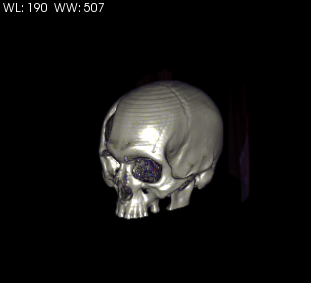
\includegraphics[width=0.33\textwidth]{raycasting_add_1}}                
  \hfill
  \subfloat[Muscle]{\label{fig:raycasting_add_2}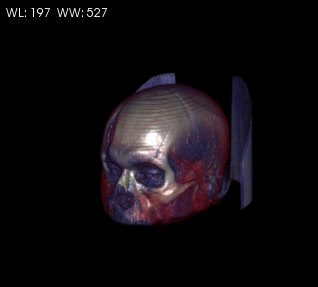
\includegraphics[width=0.333\textwidth]{raycasting_add_2}}	
  \hfill  
  \subfloat[Skin]{\label{fig:raycasting_add_3}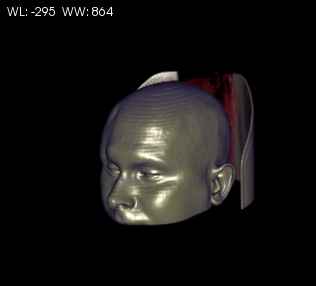
\includegraphics[width=0.332\textwidth]{raycasting_add_3}}
  \caption{Tissue Addition}
  \label{fig:raycasting_add}
\end{figure}

\newpage

\section{Cut}

In volume rendering, the cut function is used to view a cross-section of a region. With a volume pattern selected, click \textbf{Tools}, and then click \textbf{Cut plane} (Figure~\ref{fig:activate_cut_plane}).

\begin{figure}[!htb]
\centering
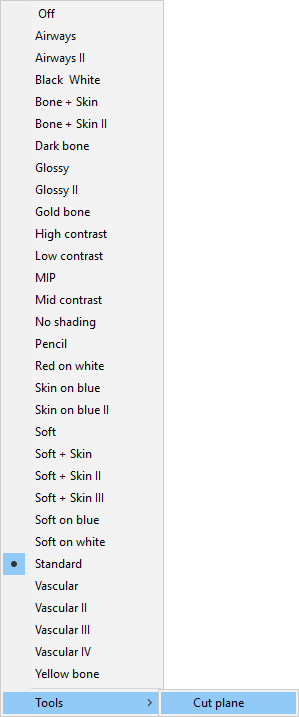
\includegraphics[scale=0.4]{activate_cut_plane_en.png}
\caption{Enabling plan to cut}
\label{fig:activate_cut_plane}
\end{figure}

An outline for cutting appears next to the volume. To make the cut, hold the left mouse button on the plane and drag the mouse. To rotate the plane, hold the left mouse button pressed on its edge and move the mouse in the desired direction as shown in Figure~\ref{fig:cutted_image}.

\begin{figure}[!htb]
\centering
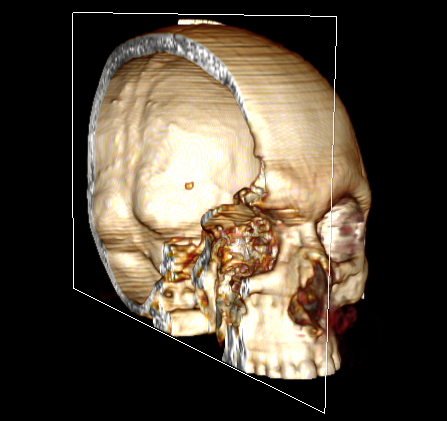
\includegraphics[scale=0.6]{cutted_image}
\caption{Image with clipping plane}
\label{fig:cutted_image}
\end{figure}

When finished using the function, click \textbf{Tools} and again click \textbf{Cut plane} (Figure~\ref{fig:cutted_image}).